\documentclass{standalone}
\usepackage{tikz}
\usepackage{ctex,siunitx}
\setCJKmainfont{Noto Serif CJK SC}
\usepackage{tkz-euclide}
\usepackage{amsmath}
\usetikzlibrary{patterns, calc}
\usetikzlibrary {decorations.pathmorphing, decorations.pathreplacing, decorations.shapes,}

\begin{document}
\small
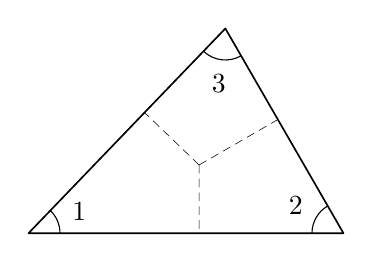
\begin{tikzpicture}[>=stealth,scale=1]
  \tkzSetUpPoint[fill=black]
  % \useasboundingbox(-1,-0.75)rectangle(3.7,1.4);
  \tkzDefPoints{0/0/B, 4/0/C, 2.5/2.6/A}
  \tkzDefTriangleCenter[centroid](A,B,C) \tkzGetPoint{G}
  \tkzDefPointBy[projection = onto  B--C](G) \tkzGetPoint{D}
  \tkzDefPointBy[projection = onto  B--A](G) \tkzGetPoint{F}
  \tkzDefPointBy[projection = onto  A--C](G) \tkzGetPoint{E}
  \tkzDrawPolygon[semithick](A,B,C)
  \tkzDrawSegments[densely dashed](G,D G,F G,E)
  \tkzMarkAngle[size=0.4](B,A,C)
  \tkzLabelAngle[pos=0.7](B,A,C){3}
  \tkzMarkAngle[size=0.4](C,B,A)
  \tkzLabelAngle[pos=0.7](C,B,A){1}
  \tkzMarkAngle[size=0.4](A,C,B)
  \tkzLabelAngle[pos=0.7](A,C,B){2}
\end{tikzpicture}
\end{document}